\begin{figure}
%\hspace*{-0.25in}\centering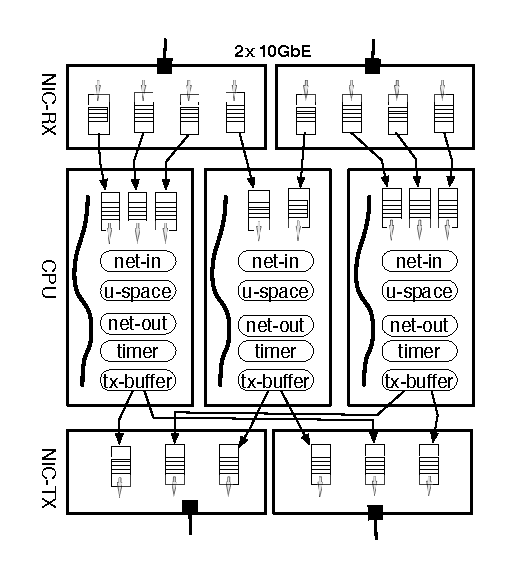
\includegraphics{figs/queues-cores.eps}
\centering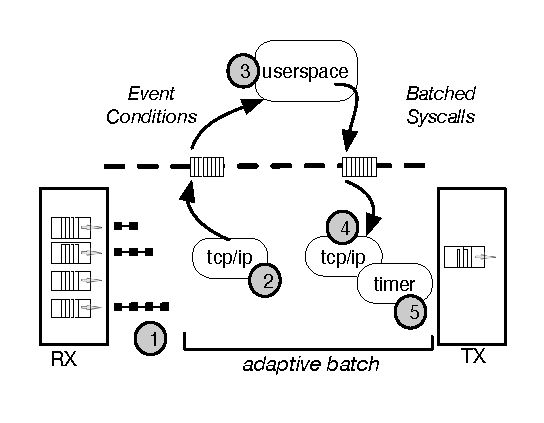
\includegraphics{figs/pipeline}
\caption{The IX pipeline. \dm{Make clear how this corresponds to
    figure 1---i.e., that the dotted line separates ring 3 from VMX
    non-root ring0.  Also, this diagram makes it look like there are
    big queues, contradicting the process to completion idea.  Maybe
    use a different abstraction for queues vs.\ batches (which I
    assume is what is being depicted across the dotted line).  Finally
    the diagram should close the loop in some way.  I.e., do you go
    straight from 5 (really 6 should be depicted0 back to 1, or do you
    invoke a scheduler or check if you need to relinquish the core at
    that point?}}
\label{fig:queues-cores}
\end{figure}

